\documentclass[10pt,conference]{IEEEtran}

\IEEEoverridecommandlockouts

\usepackage{cite}
\usepackage{amsmath,amssymb,amsfonts}
\usepackage{graphicx}
\usepackage{booktabs}
\usepackage[ruled,vlined]{algorithm2e}
\usepackage{siunitx}
\usepackage{multirow}
\usepackage{array}
\usepackage{float}
\usepackage{enumitem}
\usepackage{listings}
\usepackage{xcolor}
\usepackage{pifont}
\usepackage[normalem]{ulem}
\usepackage{soul}
\usepackage{xspace}
\usepackage{url}



\lstset{
  basicstyle=\ttfamily\footnotesize,
  keywordstyle=\color{blue},
  commentstyle=\color{gray},
  stringstyle=\color{red},
  numbers=left,
  numberstyle=\tiny,
  numbersep=5pt,
  xleftmargin=2em,
  framexleftmargin=1.5em,
  breaklines=true,
  breakatwhitespace=true,
  breakindent=0pt,
  columns=fullflexible,
  keepspaces=true,
  frame=single,
  framerule=0.4pt,
  showstringspaces=false,
  captionpos=b
}

\newcommand{\ourmethod}{\textsc{CogPath}}
\newcommand{\eg}{e.g.\xspace}
\newcommand{\xtz}[1]{\textcolor{blue}{[xtz:#1]}}
\newcommand{\ulbf}[1]{\uline{\textbf{#1}}}

\begin{document}

\title{CogPath: A Constraint-Guided Context-Reduction Framework for LLM-Based Test Generation}

\author{
\IEEEauthorblockN{Jianhan Liu, Tangzhi Xu, Yuan Yao, Feng Xu, Xiaoxing Ma}
\IEEEauthorblockA{\textit{State Key Laboratory for Novel Software Technology, Nanjing University}\\
Nanjing, China\\
\{jh.liu, xutz\}@smail.nju.edu.cn, \{y.yao, xf, xxm\}@nju.edu.cn}
}

% Copyright type CONFIRMED = standard IEEE Copyright Transfer (eCF Paper Id 1786276976373,
% signed 2026-08-09), so the "\copyright 2026 IEEE" variant below is the correct one.
% TODO: replace 979-8-XXXX-XXXX-X with the conference proceedings ISBN from the SCAM 2026
% CPS Author Kit "Preparation Instructions" (it is NOT in the eCopyright receipt).
\IEEEpubid{\makebox[\columnwidth]{979-8-XXXX-XXXX-X/26/\$31.00~\copyright2026 IEEE\hfill}%
  \hspace{\columnsep}\makebox[\columnwidth]{}}

\maketitle

%%
%% The abstract is a short summary of the work to be presented in the
%% article.
\begin{abstract}
Large language models (LLMs) have shown promise in automated unit test generation, yet achieving high branch coverage for complex methods remains challenging. 
We attribute this limitation not to model capability alone, but to a fundamental cognitive misalignment between what LLM prompts expose and what branch reachability requires: implicit cross-method preconditions are hidden, while branch-irrelevant code is over-provided. 
To address this misalignment, we propose \textsc{CogPath}, a unit test generation %constraint-guided context-reduction 
framework that externalizes hidden path conditions as Constraint-Hints and isolates branch-relevant dependencies via coverage-driven Backward Slicing, within an iterative generate–execute–repair loop. 
Our empirical evaluation, conducted on 2971 methods with cyclomatic complexity greater than 10 from 14 open-source projects, demonstrates that \textsc{CogPath} achieves 12.8\% higher line coverage and 10.2\% higher branch coverage compared to the state-of-the-art, with improvements reaching 32.3\% and 20\% respectively on the most complex project.

\end{abstract}

%%
%% The code below is generated by the tool at http://dl.acm.org/ccs.cfm.
%% Please copy and paste the code instead of the example below.
%%
% \begin{CCSXML}
% <ccs2012>
%  <concept>
%   <concept_id>00000000.0000000.0000000</concept_id>
%   <concept_desc>Do Not Use This Code, Generate the Correct Terms for Your Paper</concept_desc>
%   <concept_significance>500</concept_significance>
%  </concept>
%  <concept>
%   <concept_id>00000000.00000000.00000000</concept_id>
%   <concept_desc>Do Not Use This Code, Generate the Correct Terms for Your Paper</concept_desc>
%   <concept_significance>300</concept_significance>
%  </concept>
%  <concept>
%   <concept_id>00000000.00000000.00000000</concept_id>
%   <concept_desc>Do Not Use This Code, Generate the Correct Terms for Your Paper</concept_desc>
%   <concept_significance>100</concept_significance>
%  </concept>
%  <concept>
%   <concept_id>00000000.00000000.00000000</concept_id>
%   <concept_desc>Do Not Use This Code, Generate the Correct Terms for Your Paper</concept_desc>
%   <concept_significance>100</concept_significance>
%  </concept>
% </ccs2012>
% \end{CCSXML}

% \ccsdesc[500]{Do Not Use This Code~Generate the Correct Terms for Your Paper}
% \ccsdesc[300]{Do Not Use This Code~Generate the Correct Terms for Your Paper}
% \ccsdesc{Do Not Use This Code~Generate the Correct Terms for Your Paper}
% \ccsdesc[100]{Do Not Use This Code~Generate the Correct Terms for Your Paper}

%%
%% Keywords. The author(s) should pick words that accurately describe
%% the work being presented. Separate the keywords with commas.
\keywords{Unit Test Generation, Large Language Models, Software Testing, Program Slicing}

\section{INTRODUCTION}

Automated unit test generation plays a critical role in improving software reliability and reducing developer effort. Traditional techniques, such as symbolic execution and search-based software testing (SBST), have made substantial progress in systematically exploring input spaces and maximizing structural coverage~\cite{cadar2008klee, evosuite, mcminn2011}. However, these approaches often face fundamental limitations in scalability and in handling complex program semantics. In particular, they struggle to capture implicit preconditions that arise from intricate object states and inter-procedural interactions, where the conditions required to reach a target path are established outside the local method scope through sequences of prior method calls~\cite{baldoni2018surveysymbolicexecutiontechniques}.

Recent advances in large language models (LLMs) have introduced a new paradigm for unit test generation. By leveraging their strong code understanding and reasoning capabilities, LLM-based approaches can directly synthesize executable test cases from source code, significantly lowering the barrier to automated testing~\cite{chen2024, ryan2024, wang2024c, gu2025a, liao2025}. Moreover, iterative workflows that incorporate compilation and execution feedback have further improved the validity and coverage of generated tests~\cite{pizzorno2024}.

Despite these promising results, existing LLM-based methods still exhibit a fundamental limitation: they lack precise reasoning about \emph{implicit program constraints}, particularly those that span across multiple methods. Most approaches rely on prompting the LLM with the entire method body, optionally augmented with control-flow or type information. However, in real-world object-oriented programs, the conditions required to execute a target branch are often not locally visible within the method under test. Instead, they depend on object states established through prior method calls or initialization sequences, which are external to the focal method. As a result, LLMs frequently generate tests that are syntactically correct but fail to satisfy the hidden preconditions necessary for reaching uncovered branches~\cite{ryan2024}.

Furthermore, providing the full method body as context introduces substantial noise. Irrelevant statements consume the limited context window and obscure the critical dependencies that govern branch reachability. This not only increases the cognitive burden on the LLM but also reduces its ability to infer correct execution conditions. Consequently, even when guided by path information, existing approaches often fail to cover branches that require precise state construction, as LLM performance has been shown to degrade significantly as input context length increases, even in the absence of distracting information~\cite{du2025contextlengthhurtsllm, wang2026intelligencedegradationlongcontextllms}.

To address these challenges, we propose \ourmethod{}, a novel LLM-driven framework for automated unit test generation that tightly integrates program analysis with language model reasoning. The key idea is to reduce the difficulty of test generation from two complementary perspectives: \emph{making hidden constraints explicit} and \emph{eliminating irrelevant context}.

First, we introduce \textit{Constraints-Hints}, a mechanism that extracts path conditions from the control-flow graph and translates them into explicit, human-interpretable input requirements. Instead of requiring the LLM to infer complex branch predicates from raw source code, our approach directly exposes the necessary conditions for covering a target path, enabling more accurate and guided test generation.

Second, we propose a \textit{coverage-driven backward slicing} technique that identifies the minimal subset of program statements relevant to an uncovered branch. By focusing only on statements that influence the target condition—including cross-method dependencies such as field initialization and setter methods—the resulting slice provides a concise and semantically meaningful context for the LLM.

These two components are integrated into an iterative framework that combines test generation, execution, and automated repair. Starting from an initial test suite, the framework continuously identifies uncovered paths, derives constraint hints, and generates candidate tests. When coverage improvement stagnates, backward slicing is triggered to provide more precise guidance. This iterative feedback loop enables sustained coverage growth and effective exploration of hard-to-reach program paths.

We evaluate \ourmethod{} on a set of real-world Java projects and compare it against state-of-the-art LLM-based and search-based baselines. The results show that our approach consistently achieves higher branch coverage and is particularly effective in scenarios involving complex object state dependencies. Further analysis demonstrates that both constraint hints and backward slicing are essential for guiding LLMs toward generating semantically correct and coverage-effective tests.

In summary, this paper makes the following contributions:

\begin{itemize}[leftmargin=*]
\item We identify a key limitation of existing LLM-based test generation approaches in handling implicit, cross-method constraints.
\item We propose \textit{Constraints-Hints}, a mechanism that makes path conditions explicit and guides LLM reasoning.
\item We introduce a coverage-driven backward slicing technique to eliminate irrelevant context and expose critical dependencies.
\item We design an iterative framework that integrates generation, execution feedback, and repair for sustained coverage improvement.
\item We empirically demonstrate the effectiveness of our approach on real-world software systems.
\end{itemize}

\section{MOTIVATION}

Recent LLM-based unit test generation approaches, such as SymPrompt~\cite{ryan2024}, HITS~\cite{wang2024c}, Panta~\cite{gu2025a}, and JunitGenie~\cite{liao2025}, have achieved remarkable progress in automating test generation for complex methods, significantly reducing the manual effort required from developers. However, when the reachability of a target branch depends on \textit{object states established by prior method calls}, existing approaches still struggle to guide LLMs in constructing the appropriate external context, even when augmented with CFG-based path analysis.

The fundamental limitation is that these approaches typically supply the \textit{entire method body} as the LLM's input context. In real-world projects, however, the conditions necessary to reach a target branch are often not visible within the method body itself—they are implicit in a sequence of initialization and state-setting operations that must occur \textit{before} the method is invoked~\cite{baldoni2018surveysymbolicexecutiontechniques}. The irrelevant statements in the method body not only consume the context window but also obscure these cross-method dependencies, leaving the LLM unable to infer the required preconditions.

\textbf{A Motivating Example.}
Consider the \texttt{addValue()} method from Apache Commons 
Math~\cite{commonsMath}, shown in Listing~\ref{lst:motivation}.

\begin{lstlisting}[language=Java, 
                   caption={Target branch example from Apache Commons Math},
                   label={lst:motivation}]
// org.apache.commons.math3.stat.descriptive.SummaryStatistics
public void addValue(double value) {
    sumImpl.increment(value);
    ...
    
    if (meanImpl != mean) {   // target branch
        meanImpl.increment(value);
    }
    ...
    n++;
}
\end{lstlisting}

Suppose a test generation tool identifies that the branch at line~9 
(\texttt{meanImpl != mean}) has not been covered and attempts to generate 
a test to reach it. Existing approaches typically provide the entire method 
body alongside CFG path information to the LLM. However, the LLM faces a 
critical inferential barrier: the condition \texttt{meanImpl != mean} can 
only be satisfied if \texttt{setMeanImpl()} was called \textit{prior} to 
\texttt{addValue()}—a dependency that is entirely absent from the method 
body. Consequently, the LLM tends to generate a test such as:

\begin{lstlisting}[language=Java, caption={Typical LLM-generated test (target branch unreachable)}]
// meanImpl == mean always holds; target branch is never triggered
SummaryStatistics stats = new SummaryStatistics();
stats.addValue(1.0);
\end{lstlisting}

This test compiles and executes without error, yet the target branch is 
never triggered. The correct test requires establishing the necessary 
precondition \textit{before} invoking \texttt{addValue()}:

\begin{lstlisting}[language=Java, caption={Correct test (target branch reachable)}]
// Establish precondition via setMeanImpl() before calling addValue()
SummaryStatistics stats = new SummaryStatistics();
stats.setMeanImpl(new CustomMeanImpl()); // makes meanImpl != mean
stats.addValue(1.0);                     // target branch now reachable
\end{lstlisting}

This example illustrates two core challenges that existing approaches fail 
to address: \textbf{(1)} the method body contains numerous statements 
irrelevant to the target branch, which dilute the LLM's attention and 
impede precise reasoning; and \textbf{(2)} the true precondition for 
reaching the target branch is a cross-method dependency invisible within 
the method body itself.

\textbf{Our Approach.}
To address these challenges, we propose two complementary mechanisms that 
reduce LLM reasoning complexity from the perspectives of 
\textit{information reduction} and \textit{condition explicitness}:

\begin{itemize}[leftmargin=*]
    \item \textbf{Backward Slicing.} Starting from the target branch condition
    \texttt{meanImpl != mean}, we perform backward slicing to trace all
    statements with data or control dependencies on \texttt{meanImpl} and
    \texttt{mean}, including field declarations, default assignments in the
    constructor, and the definition of \texttt{setMeanImpl()}. This eliminates
    six irrelevant \texttt{increment} calls and other unrelated branches from
    the context, allowing the LLM to focus on statements that govern branch
    reachability.

    \item \textbf{Constraint Hints.} Building on the slice, we explicitly
    provide the LLM with the path condition and how it can be established,
    e.g., \emph{``To trigger the target branch, \texttt{meanImpl != mean} must
    hold; this can be achieved by calling \texttt{setMeanImpl(customImpl)}
    before \texttt{addValue()}.''} Rather than requiring the LLM to infer
    implicit cross-method dependencies from source code, this mechanism
    directly guides the LLM toward constructing the correct initialization
    sequence.
\end{itemize}

Together, these two mechanisms systematically reduce the difficulty of 
reasoning about complex branch conditions, enabling LLMs to generate tests 
that reach previously uncovered paths.

\section{Methodology}

\subsection{Overview}

\begin{figure*}[t]
\centering
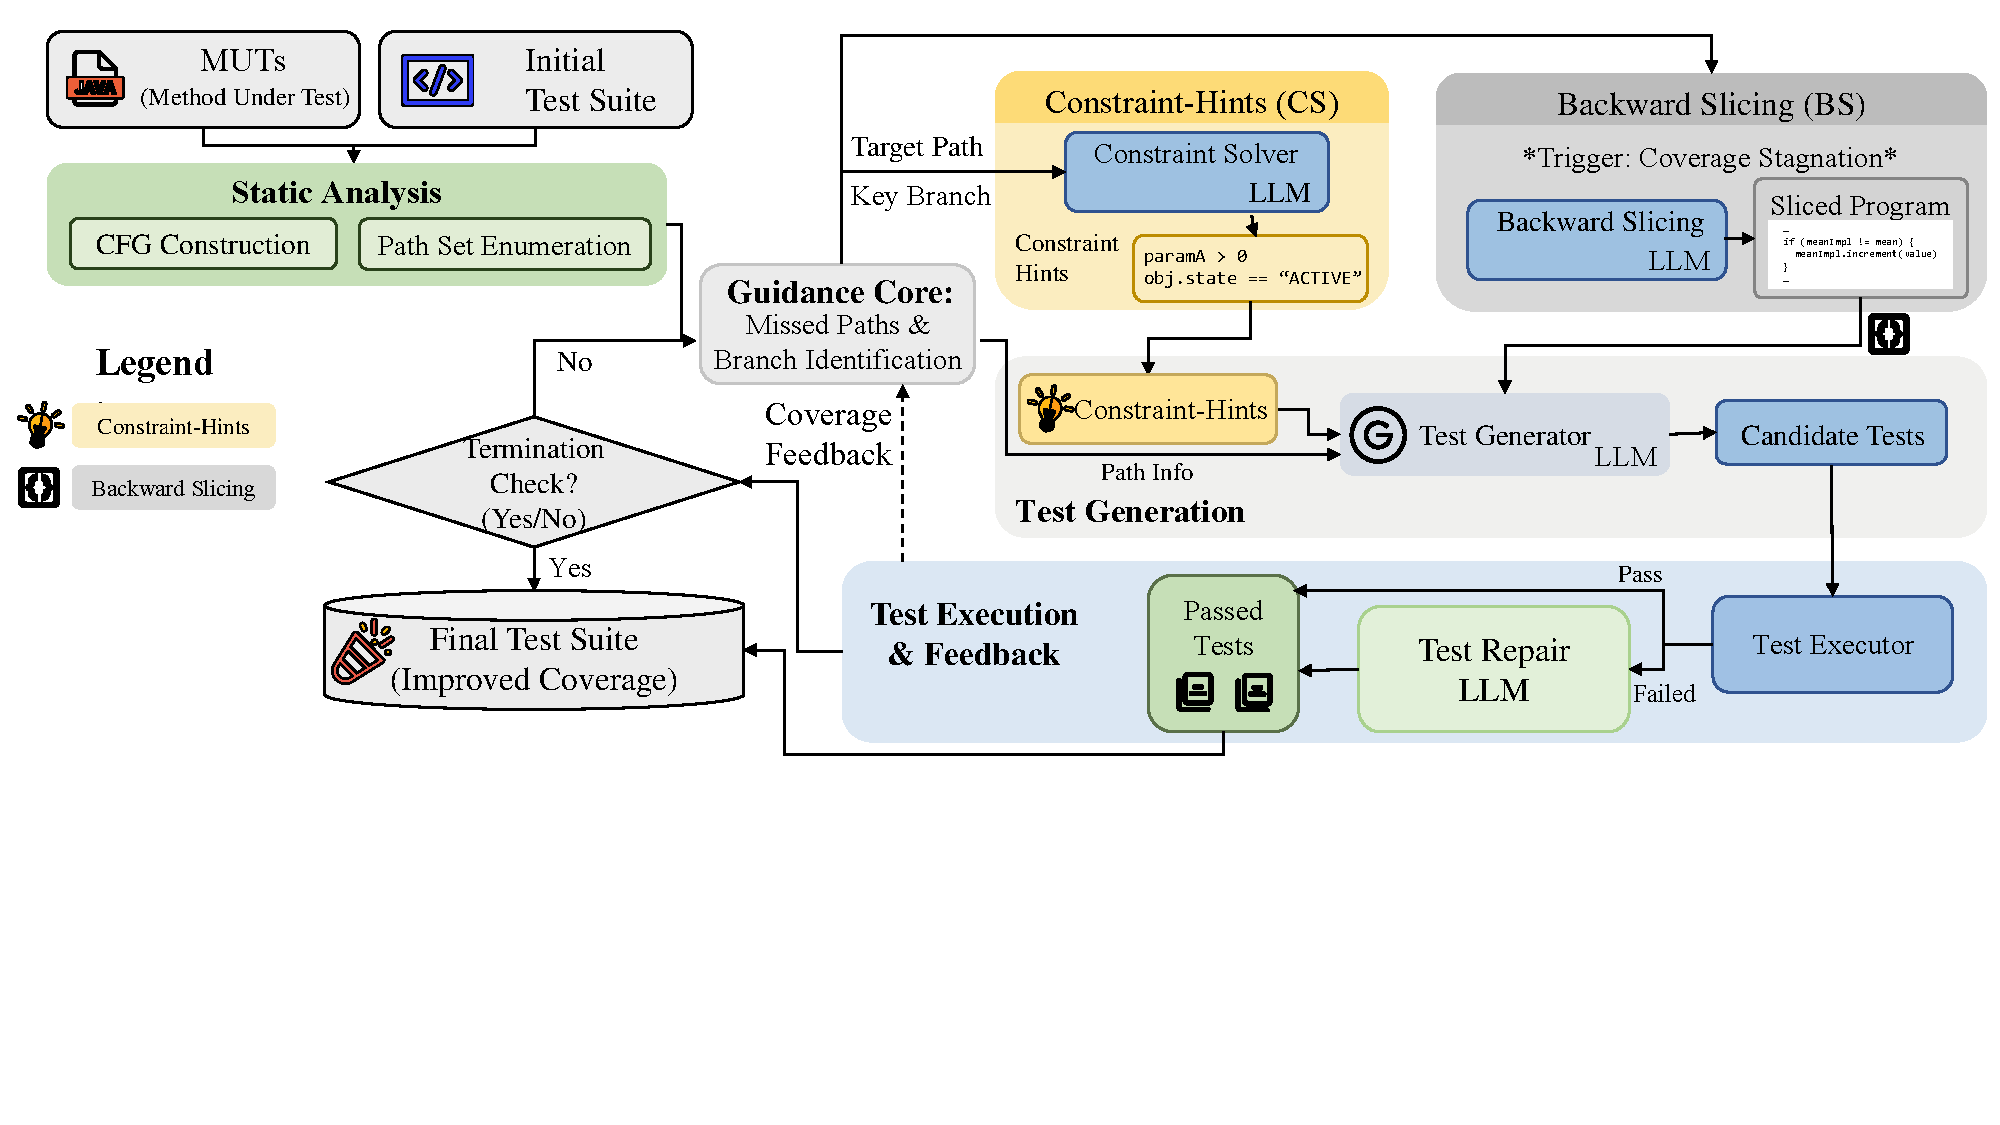
\includegraphics[width=\linewidth]{figures/overview.pdf}
\caption{Overview of the coverage-guided test generation framework.}
\label{fig:overview}
\end{figure*}

\ourmethod{} is a coverage-guided iterative framework for automated unit test generation, illustrated in Figure~\ref{fig:overview}.Given a method under test, \ourmethod{} first performs an initialization step that extracts project-level dependencies, resolves the required JUnit imports, and seeds the suite with a syntactically valid scaffolding test containing a trivial \texttt{assertTrue(true)} assertion, ensuring a compilable starting point for all subsequent iterations.It then constructs the CFG, enumerates feasible paths, and collects dynamic coverage feedback to identify uncovered branches before entering an iterative refinement loop.

Each iteration begins with path selection, where \textit{Constraint-Hints} analyzes the selected uncovered path and injects explicit branch conditions as structured guidance into the generation prompt.When coverage improvement stagnates, \textit{Backward Slicing} is activated, replacing the full method body with the minimal set of statements that bear data or control dependence on the target branch.The LLM then generates candidate tests against this focused context; passing tests are merged into the suite while failing ones are forwarded to the repair phase.During repair, compiler diagnostics—including error messages and their associated line numbers—are incorporated into the repair prompt, allowing the LLM to precisely locate and correct the offending statements rather than re-generating the test from scratch.Coverage is re-measured at the end of each iteration to drive target selection in the next round.The loop terminates when the coverage target is reached, the iteration budget is exhausted, or coverage fails to improve for a configurable number of consecutive iterations.

\subsection{Constraints-Hints}

\textit{Constraints-Hints} addresses the implicit precondition problem by 
decoupling constraint inference from test synthesis. Instead of requiring 
the LLM to simultaneously infer branch reachability and generate tests, 
we explicitly extract the conditions necessary to trigger a target branch 
and provide them as structured guidance.

While symbolic execution can derive precise path conditions, it often 
struggles to scale to real-world programs due to path explosion, complex 
heap interactions, and challenges in modeling external libraries and 
reflection~\cite{baldoni2018, cadar2008klee}. 
Rather than performing exact constraint solving, we aim to extract 
\emph{sufficient} conditions that characterize branch reachability.

Concretely, given an uncovered branch, we analyze its predicate and 
derive a set of constraint hints that describe the required program state 
(e.g., variable relations, nullness conditions, and key object properties). 
These hints are then embedded into the generation prompt, guiding the LLM 
to construct inputs and invocation sequences that satisfy the target condition.

By transforming implicit dependencies into explicit guidance, 
\textit{Constraints-Hints} reduces the reasoning burden on the LLM and 
enables more reliable generation of tests that reach previously uncovered branches.

\paragraph{Path formulation.}

Let $P = \langle b_1, b_2, \ldots, b_k \rangle$ denote the sequence of branch
decisions along a target execution path $\pi$, where each predicate
$b_i(\mathbf{x}) \in \{\texttt{true}, \texttt{false}\}$ is evaluated over the
program input vector $\mathbf{x}$. Covering the path requires an input
assignment $\mathbf{x}^*$ that satisfies all branch predicates along the
path:

\begin{equation}
\mathbf{x}^* \in \mathcal{F}(\pi) =
\left\{
\mathbf{x} \mid
b_1(\mathbf{x}) \wedge b_2(\mathbf{x}) \wedge \cdots \wedge b_k(\mathbf{x})
\right\}.
\end{equation}

Rather than solving this constraint system symbolically—which can be
computationally expensive and brittle under complex object states or
indirect method calls—\ourmethod{} employs an LLM-based constraint solver to
approximate the feasible input space as a lightweight set of interpretable conditions:

\begin{equation}
\mathcal{C}(\pi) =
\left\{
c_j \mid
c_j \text{ is a necessary condition on } \mathbf{x}
\right\}.
\end{equation}

The first uncovered branch along the path, denoted as $b^*$, is identified
from the coverage report and provided to the solver as additional context,
guiding the model toward the most immediate obstacle preventing the path
from being executed.

\paragraph{Integration.}

The constraint-solving prompt is generated from a configurable template that
incorporates the source code, the branch sequence of $\pi$, and the uncovered
branch $b^*$. The solver produces $\mathcal{C}(\pi)$ as a list of conditions
such as \texttt{paramA > 0} or \texttt{obj.status == "ACTIVE"}. These
conditions are appended to the test generation prompt, transforming an
opaque path coverage objective into a concrete specification of required
inputs.

\paragraph{Example.}

Consider the \texttt{addValue} method, which contains three conditional
branches dispatching to overridable statistical implementations. An
existing test suite covers only the false branches of all three predicates,
meaning \texttt{meanImpl}, \texttt{varianceImpl}, and \texttt{geoMeanImpl}
all refer to their default implementations. The first uncovered branch is
\texttt{(meanImpl != mean)}. The constraint solver identifies that
satisfying this predicate requires replacing the default implementation
before invoking \texttt{addValue}. This object-state precondition is
expressed as a constraint in $\mathcal{C}(\pi)$:

\[
c : \texttt{meanImpl} \neq \texttt{mean}
\]

which implies that a call such as \texttt{setMeanImpl(...)} must occur prior
to invoking \texttt{addValue}. By making this requirement explicit, the test
generation LLM can construct the correct setup sequence and cover the
previously unreachable branch.

\subsection{Backward Slicing}

Coverage improvement does not always progress smoothly: certain branches remain persistently uncovered even after multiple iterations, typically because their reachability depends on subtle state dependencies that standard generation fails to capture. 
When such a plateau is detected, \ourmethod{} triggers a backward slicing step targeted at these stubborn branches, replacing the full method body with the minimal context actually relevant to the uncovered path.

\paragraph{Slice extraction.}

Given an uncovered path $\pi$, the framework extracts the subset of statements that may influence the execution of that path:

\begin{equation}
\textit{Slice}(P,\pi) =
\left\{
s_i \in P \mid s_i \rightsquigarrow \pi
\right\}.
\end{equation}

A dedicated LLM is then invoked with the uncovered code segment, the focal method source code, and dependency context from related classes. The model returns a structured response containing the relevant slice statements, required input values, necessary object states, and potential setup operations.

\paragraph{Test generation from slices.}

The extracted slice information is supplied as additional context to the test generation prompt. The LLM then generates targeted unit tests that incorporate the identified prerequisites directly. These tests are compiled, executed, and measured using the same validation pipeline as regular test candidates, allowing the framework to recover from coverage plateaus while maintaining the overall iterative workflow.

\subsection{Iterative Workflow of \ourmethod{}}

\begin{algorithm}[t]
\small
\caption{Iterative Test Generation with Constraints-Hints and Backward Slicing}
\label{alg:main}
\SetAlgoLined
\KwIn{$\textit{src}$: source file, $\textit{suite}$: initial test suite (possibly empty)}
\KwOut{Augmented test suite with improved coverage}

$\textit{deps} \leftarrow \textsc{ExtractDeps}()$\;
$\textit{cfg}, \textit{methodDict} \leftarrow \textsc{BuildCFG}(\textit{src})$\;
$\textit{noIncr} \leftarrow 0$, \quad $\textit{iter} \leftarrow 0$\;
$\textit{cov}, \textit{missed} \leftarrow \textsc{RunCoverage}(\textit{suite})$\;

\While{$\textit{iter} < \textit{maxIter}$ \textbf{and} $\textit{noIncr} < \Lambda$ \textbf{and} $\textit{cov} < \tau$}{

    \tcp{Path selection and prompt construction}
    \eIf{$\textit{cov} = 0$ \textbf{or} $\textit{iter} = 0$}{
        $\textit{prompt} \leftarrow \textsc{BuildBaselinePrompt}(\textit{src}, \textit{suite}, \textit{deps})$\; \tcp*[r]{baseline prompt}
    }{
        $\Pi \leftarrow \textsc{SelectPaths}(\textit{cfg}, \textit{methodDict}, \textit{missed})$\;
        $\mathcal{C} \leftarrow \emptyset$\;
        \ForEach{path $\pi \in \Pi$}{
            $b^* \leftarrow \textsc{FirstUncoveredBranch}(\pi, \textit{missed})$\;
            $\mathcal{C}(\pi) \leftarrow \textsc{ConstraintSolver}(\textit{src}, \pi, b^*)$\; \tcp*[r]{Constraints-Hints}
        }
        $\textit{prompt} \leftarrow \textsc{BuildPrompt}(\textit{src}, \textit{suite}, \textit{deps}, \Pi, \mathcal{C})$\;
    }

    \tcp{Test generation}
    $\mathcal{T} \leftarrow \textsc{GenerateTests}(\textit{prompt})$\;

    \tcp{Backward slicing for stubborn uncovered paths}
    \If{$\textit{noIncr} \geq \beta \cdot \Lambda$}{
        $\textit{slices} \leftarrow \textsc{BackwardSlicer}(\textit{src}, \textit{missed})$\;
        $\mathcal{T} \leftarrow \mathcal{T} \cup \textsc{GenerateFromSlices}(\textit{slices}, \textit{suite}, \textit{deps})$\;
    }

    \tcp{Validation and repair}
    $\textit{failed} \leftarrow \{\}$\;
    \ForEach{$t \in \mathcal{T}$}{
        \lIf{$\textsc{ValidateTest}(t, \textit{suite})$}{$\textit{suite} \leftarrow \textit{suite} \cup \{t\}$}
        \lElse{$\textit{failed} \leftarrow \textit{failed} \cup \{t\}$}
    }
    \If{$\textit{failed} \neq \emptyset$}{
        $\textit{suite} \leftarrow \textit{suite} \cup \textsc{RepairAndValidate}(\textit{failed}, \textit{src}, \textit{suite}, \textit{deps})$\;
    }

    \tcp{Coverage update and termination check}
    $(\textit{cov}',\, \textit{missed}') \leftarrow \textsc{RunCoverage}(\textit{suite})$\;
    \lIf{$\textit{cov}' > \textit{cov}$}{$\textit{noIncr} \leftarrow 0$}
    \lElse{$\textit{noIncr} \leftarrow \textit{noIncr} + 1$}
    $\textit{cov} \leftarrow \textit{cov}'$, \quad
    $\textit{missed} \leftarrow \textit{missed}'$, \quad
    $\textit{iter} \leftarrow \textit{iter} + 1$\;
}

\Return $\textit{suite}$\;
\end{algorithm}

The complete workflow of \ourmethod{} is formalized in Algorithm~\ref{alg:main}. The framework accepts the source file and an initial test suite as input, and iteratively generates, validates, and repairs tests until a coverage target is met or a termination condition is triggered.


\paragraph{Initialization.}
The framework extracts test-scope dependencies, constructs the CFG and method dictionary from the source file, and measures baseline coverage on the initial suite (lines 1--4).

\paragraph{Path selection with Constraints-Hints.}
At each non-initial iteration, \textsc{SelectUncoveredPaths} identifies candidate paths from the CFG that intersect with missed lines or branches, weighted by both coverage impact and visit history $\textit{pathHistory}$ (line 8). For each selected path $\pi$, the constraint solver derives $\mathcal{C}(\pi)$ by analyzing the branch sequence up to the first uncovered predicate $b^*$, and these conditions are embedded into the generation prompt (lines 9--13).

\paragraph{Backward slicing.}
When $\textit{noIncr} \geq \beta \cdot \Lambda$, indicating a coverage plateau, the backward slicer is invoked on the remaining missed code segments. It returns structured prerequisite information---required inputs, object states, and method mocks---which is used to construct an additional batch of targeted tests $\mathcal{T}_s$ (lines 16--19).

\paragraph{Validation and repair.}
Each generated test is individually inserted into the suite and executed. Failing tests are collected with their error messages and forwarded to the repair phase, which re-invokes the LLM with failure feedback to produce corrected versions. Successfully validated repaired tests are also incorporated into the suite (lines 21--32).

\paragraph{Termination.}
The loop exits when the coverage target $\tau$ is reached, the maximum iteration count $\textit{maxIter}$ is exhausted, or coverage fails to improve for $\Lambda$ consecutive iterations.


\section{EXPERIMENTS}

\begin{table*}[t]
\centering
\caption{Dataset Metrics with \#MUTs}
\label{tab:dataset}
\begin{tabular}{l l l *{5}{>{\centering\arraybackslash}p{1.4cm}}}
\toprule
\textbf{Identifier} & \textbf{Project} & \textbf{Version} & \textbf{\#C} & \textbf{\#MUTs} & \textbf{$CC_{max}$} & \textbf{$CC_{min}$} & \textbf{$CC_{med}$} \\
\midrule
Cli & Cli-40f & 1.5-SNAP & 2 & 31 & 11 & 11 & 11 \\
Codec & Codec-18f & 1.11-SNAP & 7 & 78 & 31 & 11 & 13 \\
Collections & Collections-28f & 4.2-SNAP & 5 & 218 & 32 & 11 & 16 \\
Compress & Compress-47f & 1.16-SNAP & 9 & 65 & 22 & 11 & 13 \\
Csv & Csv-16f & 1.6-SNAP & 3 & 72 & 25 & 11 & 14 \\
Gson & Gson-16f & 2.8.2-SNAP & 4 & 75 & 37 & 11 & 22 \\
JCore & JacksonCore-26f & 2.10.0-SNAP & 9 & 161 & 30 & 11 & 14 \\
JDatabind & JacksonDatabind-112f & 2.9.9 & 9 & 371 & 22 & 11 & 15 \\
JXml & JacksonXml-5f & 2.9.6-SNAP & 4 & 118 & 29 & 12 & 22 \\
Jsoup & Jsoup-93f & 1.12.2-SNAP & 8 & 171 & 22 & 11 & 12 \\
JxPath & JxPath-22f & 1.4-SNAP & 12 & 115 & 32 & 11 & 13 \\
Lang & Lang-4f & 3.2-SNAP & 17 & 586 & 30 & 11 & 16 \\
Math & Math-2f & 3.3-SNAP & 30 & 452 & 31 & 11 & 14 \\
Time & Time-13f & 2.1 & 11 & 458 & 30 & 11 & 17 \\
\midrule
Total/Avg & & & \textbf{130} & \textbf{2971}  & \textbf{27.4}  & \textbf{11.1}  & \textbf{15.1} \\
\bottomrule
\end{tabular}
\end{table*}

\subsection{Experimental Setup}

In this section, we first introduce the construction and statistics of the evaluation dataset.


\textbf{Dataset.} To evaluate the effectiveness of \ourmethod{} in generating unit tests for complex methods, we utilize real-world subjects from the Defects4J (v2.0.1) benchmark \cite{defects4j}. 
We selected the latest fixed version of each subject program to ensure compatibility with modern build environments. 
Following prior work \cite{gu2025a}, we excluded projects that do not use Maven or rely on deprecated dependencies (i.e., Chart, Mockito, and Closure). 
The remaining 14 subjects are compatible with Java 8+, Maven (v3.6.3), and JUnit (v4.13.2).
To specifically assess performance on logic-heavy code, we focus on complex classes rather than entire projects. 
We identified non-abstract, public classes containing at least one method with Cyclomatic Complexity (CC) $> 10$ \cite{mccabe1976complexity}. 
The statistics of our evaluation dataset are summarized in Table~\ref{tab:dataset}.



\textbf{Evaluation Metrics.}
To evaluate the effectiveness of the generated unit tests, we primarily focus on code coverage, which is the standard metric in automated test generation research \cite{randoop, evosuite}. We report two specific metrics:
\begin{itemize}
\item \textbf{Line Coverage (LC):} The ratio of executable lines in the target class that are exercised by the generated test suite. It provides a baseline measure of how much of the implementation has been reached.
\item \textbf{Branch Coverage (BC):} The ratio of executed decision outcomes (e.g., the true and false paths of an \textit{if} statement) to the total number of possible branches. Given our focus on methods with high Cyclomatic Complexity ($CC > 10$), branch coverage is our primary metric, as it more accurately reflects the tool's ability to navigate complex logical structures and boundary conditions.
\end{itemize}
All coverage data in our experiments are collected using the JaCoCo library, ensuring consistent and reproducible measurements across all subjects and baselines.

\textbf{Research Questions.}
To evaluate the effectiveness and design of \ourmethod{}, we address the following three research questions:

\begin{itemize}
\item \textbf{RQ1: Effectiveness Comparison.} How does \ourmethod{} perform compared to state-of-the-art LLM-based test generation approaches in terms of line and branch coverage on complex, logic-heavy methods?
\item \textbf{RQ2: Contribution of Components.} What are the individual contributions of the Backward Slicing (BS) and Constraint Solver (CS) components to the overall performance of \ourmethod{}?
\item \textbf{RQ3: Model Generalizability.} Is \ourmethod{}'s effectiveness robust across different underlying Large Language Models, and how do their performances vary?
\end{itemize}

\textbf{Baselines.}
To evaluate the performance of \ourmethod{}, we compare it against three state-of-the-art LLM-based unit test generation frameworks representing diverse paradigms in the field:

\begin{itemize}
    \item \textbf{SymPrompt \cite{ryan2024}:} A prompt-engineering approach that encodes symbolic execution concepts into structured prompts. It extracts branch conditions from Control Flow Graphs CFGs) and constructs path-oriented prompts to guide the LLM in generating inputs that satisfy specific execution paths.
    \item \textbf{HITS \cite{wang2024c}:} A hierarchical prompting framework that decomposes complex methods into smaller code segments before test generation. It adopts a self-healing strategy that iteratively repairs failing tests to improve compilability and coverage.
    \item \textbf{Panta \cite{gu2025a}:} A hybrid framework that combines static CFG analysis with dynamic coverage feedback to identify uncovered paths. It constructs context-aware prompts that expose intra-class data dependencies to guide the LLM toward uncovered branches.
\end{itemize}

Due to missing components in the official HITS repository, we re-implemented its workflow by strictly following the prompt templates described in the paper and the procedural logic of available open-source fragments. For fair comparison, all methods use the same backbone model as \ourmethod{} in each experiment. In RQ1 and RQ2, we adopt Qwen3-Coder-30B (QC3-30B), deployed locally on an NVIDIA H800 GPU (80\,GB) for cost-efficient evaluation, while RQ3 further includes Qwen3.5-397B-A17B, GPT-5.4-Mini, and DeepSeek-V3.1 to assess generalizability. For each MUT, all approaches are restricted to the declaring class source code and import statements, without access to project-level dependencies or configurations, ensuring that performance differences stem from the frameworks rather than external information. To improve reproducibility, all models are configured with temperature $0.2$ and top-$p$ $1.0$. The key hyperparameters of \ourmethod{} are set as follows: $\textit{maxIter}=20$, $\Lambda=3$, $\beta=0.6$, and target coverage $\tau=100.00\%$, with all experiments starting from an empty test suite.

\begin{table*}[t]
\centering
\caption{Coverage Across Approaches}
\label{tab:coverage}
\small
\sisetup{round-mode=places, round-precision=2, table-format=2.2}
\begin{tabular}{@{} l c c *{10}{S[table-column-width=1.1cm]} @{}}
\toprule
\multirow{2}{*}{Project} & \multirow{2}{*}{\#C} & \multirow{2}{*}{$CC_{avg}$} & 
\multicolumn{2}{c}{Vanilla Prompt} &
\multicolumn{2}{c}{SymPrompt} & \multicolumn{2}{c}{HITS} & \multicolumn{2}{c}{Panta} & \multicolumn{2}{c}{\ourmethod{}} \\
\cmidrule(lr){4-5} \cmidrule(lr){6-7} \cmidrule(lr){8-9} \cmidrule(lr){10-11} \cmidrule(lr){12-13}
 & & & {LC(\%)} & {BC(\%)} & {LC(\%)} & {BC(\%)} & {LC(\%)} & {BC(\%)} & {LC(\%)} & {BC(\%)} & {LC(\%)} & {BC(\%)} \\
\midrule
Cli         & 2  & 11.00 & 36.81 & 31.99 & 17.93 & 9.02  & 73.50          & 59.58          & 63.11          & 37.98          & \bf{84.32} & \bf{70.73} \\
Codec       & 7  & 16.14 & 24.58 & 21.96 & 29.68 & 24.96 & 65.73          & 60.25          & 60.53          & 54.82          & \bf{76.97} & \bf{69.60} \\
Collections & 5  & 18.60 & 8.38  & 6.72  & 32.63 & 32.42 & \bf{68.23}     & \bf{70.00}     & 33.44          & 32.40          & 40.46      & 34.63      \\
Compress    & 9  & 15.33 & 7.49  & 4.31  & 11.84 & 11.34 & 31.64          & 25.24          & 34.36          & 28.45          & \bf{36.09} & \bf{29.05} \\
Csv         & 3  & 16.67 & 25.22 & 14.46 & 37.69 & 23.79 & 28.95          & 14.73          & 50.98          & 37.99          & \bf{62.27} & \bf{52.29} \\
Gson        & 4  & 23.25 & 12.78 & 2.32  & 13.16 & 3.59  & 31.54          & 21.25          & 21.81          & 15.20          & \bf{63.82} & \bf{41.24} \\
JCore       & 9  & 16.33 & 19.44 & 15.13 & 23.62 & 21.44 & 19.85          & 18.51          & 26.24          & 21.97          & \bf{41.72} & \bf{35.54} \\
JDatabind   & 9  & 15.33 & 7.95  & 4.98  & 9.99  & 6.06  & 18.33          & 14.44          & 18.17          & 14.34          & \bf{23.35} & \bf{17.85} \\
JXml        & 4  & 21.50 & 19.13 & 14.86 & 17.45 & 18.56 & 18.59          & 18.84          & \bf{31.89}     & \bf{23.55}     & 20.61      & 17.08      \\
Jsoup       & 8  & 14.13 & 27.30 & 17.94 & 24.72 & 19.13 & 27.82          & 17.36          & 49.80          & 39.25          & \bf{66.43} & \bf{52.55} \\
JxPath      & 12 & 15.50 & 17.66 & 12.19 & 12.01 & 9.48  & 23.11          & 22.76          & 34.10          & 29.35          & \bf{42.28} & \bf{35.84} \\
Lang        & 17 & 16.88 & 21.35 & 17.10 & 43.98 & 40.42 & \bf{62.82}     & \bf{59.77}     & 39.26          & 36.61          & 59.21      & 52.14      \\
Math        & 30 & 16.47 & 25.27 & 20.83 & 38.55 & 33.70 & 30.87          & 26.38          & 46.40          & 39.16          & \bf{59.60} & \bf{54.02} \\
Time        & 11 & 17.36 & 31.42 & 23.85 & 53.37 & 42.06 & 63.32          & 50.23          & 46.74          & 41.42          & \bf{66.79} & \bf{59.25} \\
\midrule
\multicolumn{3}{l}{Average} & 20.34 & 14.90 & 26.19 & 21.14 & 40.31 & 34.24 & 39.77 & 32.32 & \bf{53.14} & \bf{44.41} \\
\bottomrule
\end{tabular}
\end{table*}

\subsection{RQ1: Effectiveness of Our Approach}


To answer RQ1, we compare \ourmethod{} against three state-of-the-art baselines on the selected dataset. Results are summarized in Table~\ref{tab:coverage}.


\subsubsection{Overall Performance}
As shown in Table~\ref{tab:coverage}, \ourmethod{} achieves the highest average LC and BC across all projects. 
Specifically, it attains an average BC of 44.41\%, outperforming SymPrompt (21.14\%), HITS (34.24\%), and Panta (32.32\%). 

Gains over the two strongest baselines---HITS (\textbf{+10.2\%}) and Panta (\textbf{+12.1\%})---confirm that jointly reducing irrelevant context and making implicit preconditions explicit addresses coverage gaps that iterative refinement and context-aware prompting alone cannot close. 
The margin widens substantially against SymPrompt (\textbf{+23.3\%}), underscoring the necessity of explicit program analysis when navigating logic-heavy control flows.


\subsubsection{Performance on High-Complexity Projects}
The advantages of \ourmethod{} are most pronounced on projects with high cyclomatic complexity and deeper inter-method dependencies. 

For instance, on Gson (CC$_{avg}$ = 23.25, the highest in the benchmark), \ourmethod{} achieves a BC of 41.24\% while SymPrompt reaches only 3.59\%; on JCore (CC$_{avg}$ = 16.33), BC rises from 18.51\% (HITS) to 35.54\%; and on Jsoup (CC$_{avg}$ = 14.13), BC improves from 17.36\% (HITS) to 52.55\%.
These gains collectively demonstrate that reducing irrelevant context via backward slicing and surfacing implicit preconditions via constraint hints are both essential for navigating the dense branching logic and cross-method dependencies that characterize high-complexity projects.

These results indicate that \ourmethod{} excels particularly in logic-heavy methods where complex object interactions and conditional dependencies are prevalent.

\begin{tcolorbox}[colback=gray!5, colframe=gray!100, title=Answer to RQ1]
\ourmethod{} outperforms all three baselines on average, achieving a BC of 44.41\%, representing improvements of 10.2\%--23.3\% over baselines. 
Its advantage is most pronounced in projects with high cyclomatic complexity and cross-method dependencies (e.g., +20\% on Gson, +14\% on JCore).
\end{tcolorbox}



\subsection{RQ2: Ablation Study}

\begin{table*}[htbp]
\centering
\caption{Ablation Study of \ourmethod{} Components}
\label{tab:ablation}
\small
\sisetup{round-mode=places, round-precision=2, table-format=2.2}
\begin{tabular}{@{} l c *{8}{S} @{}}
\toprule
\multirow{2}{*}{Project} & \multirow{2}{*}{$CC_{avg}$} 
& \multicolumn{2}{c}{CogPath} 
& \multicolumn{2}{c}{w/o CS} 
& \multicolumn{2}{c}{w/o BS} 
& \multicolumn{2}{c}{w/o CS+BS} \\
\cmidrule(lr){3-4} \cmidrule(lr){5-6} \cmidrule(lr){7-8} \cmidrule(lr){9-10}
 & & {LC(\%)} & {BC(\%)} & {LC(\%)} & {BC(\%)} & {LC(\%)} & {BC(\%)} & {LC(\%)} & {BC(\%)} \\
\midrule
Cli               & 11.00 & 84.32 & 70.73 & 84.74 & 68.75 & 68.69 & 57.68 & 72.62 & 56.54 \\
Codec             & 16.14 & 76.97 & 69.60 & 54.86 & 50.68 & 66.77 & 57.94 & 66.34 & 56.53 \\
Collections       & 18.60 & 40.46 & 34.63 & 39.51 & 38.59 & 32.42 & 36.60 & 37.43 & 34.45 \\
Compress          & 15.33 & 36.09 & 29.05 & 31.22 & 28.58 & 25.43 & 19.04 & 23.45 & 18.11 \\
Csv               & 16.67 & 62.27 & 52.29 & 46.18 & 36.38 & 36.47 & 24.80 & 60.54 & 47.07 \\
Gson              & 23.25 & 63.82 & 41.24 & 43.94 & 27.73 & 49.40 & 31.85 & 40.92 & 26.52 \\
JCore       & 16.33 & 41.72 & 35.54 & 30.58 & 27.31 & 45.39 & 39.20 & 22.97 & 21.07 \\
JDatabind   & 15.33 & 23.35 & 17.85 & 12.44 & 9.33  & 33.74 & 26.55 & 19.59 & 15.54 \\
JXml        & 21.50 & 20.61 & 17.08 & 23.80 & 18.61 & 35.30 & 26.84 & 26.79 & 23.08 \\
Jsoup             & 14.13 & 66.43 & 52.55 & 61.48 & 46.64 & 69.11 & 53.76 & 59.00 & 47.11 \\
JxPath            & 15.50 & 42.28 & 35.84 & 47.56 & 41.96 & 28.06 & 22.35 & 34.94 & 31.44 \\
Lang              & 16.88 & 59.21 & 52.14 & 66.05 & 63.04 & 56.84 & 51.38 & 57.12 & 53.91 \\
Math              & 16.47 & 59.60 & 54.02 & 63.42 & 56.61 & 38.60 & 32.66 & 43.23 & 39.90 \\
Time              & 17.36 & 66.79 & 59.25 & 46.29 & 42.81 & 64.99 & 57.89 & 43.21 & 40.65 \\
\midrule
\multicolumn{2}{l}{Average} & \textbf{53.14} & \textbf{44.41} & 46.58 & 39.79 & 46.51 & 38.47 & 43.44 & 36.57 \\
\bottomrule
\end{tabular}
\end{table*}

To evaluate the individual contributions of Backward Slicing (BS) and Constraint Hints (CS), we conducted an ablation study with three degraded variants: \textbf{w/o BS} (removing backward slicing), \textbf{w/o CS} (removing constraint hints), and \textbf{w/o CS+BS} (removing both). All variants share the same iterative generation loop and are evaluated under an identical backbone (QC3-30B). Results are summarized in Table~\ref{tab:ablation}.

\subsubsection{Overall Ablation Results}

\textbf{Both components contribute independently.} Removing BS alone causes an average BC drop of \textbf{5.94 percentage points} (44.41\% $\to$ 38.47\%), while removing CS alone results in a drop of \textbf{4.62 pp} (44.41\% $\to$ 39.79\%). Removing both components yields the largest degradation of \textbf{7.84 pp} (44.41\% $\to$ 36.57\%), confirming that BS and CS address complementary aspects of the problem: BS eliminates irrelevant context that misleads the LLM, while CS makes cross-method preconditions explicit so that the LLM can construct the required object state. Notably, the combined degradation (7.84 pp) is smaller than the sum of individual degradations (10.56 pp), suggesting that the two components partially compensate for each other when one is absent.

\textbf{BS is particularly critical for context-heavy methods.} The impact of BS is most pronounced in projects where method bodies contain many statements unrelated to the target branch. On \textit{Csv}, removing BS causes BC to drop from 52.29\% to 24.80\% ($-$27.49 pp), the largest per-project degradation in the study. This aligns with our motivation: when irrelevant statements dominate the focal method, providing the full unsliced context actively distracts the LLM from the branch-relevant logic.

\textbf{CS is critical when preconditions span method boundaries.} CS contributes most on projects where the target branch condition depends on prior method calls. On \textit{JacksonDatabind}, removing CS reduces BC from 17.85\% to 9.33\% ($-$8.52 pp, a relative decline of 47.7\%), indicating that without explicit constraint hints the LLM is unable to construct the object state necessary to reach the focal branch.

\textbf{Anomalies and discussion.} In two projects (\textit{JacksonCore} and \textit{Jsoup}), the w/o-BS variant achieves marginally higher coverage than the full \ourmethod{}. We attribute this to cases where backward slicing inadvertently removes type information required for mock construction, causing the LLM to fall back on simpler yet occasionally effective test patterns. This sensitivity to slice granularity is a known limitation and remains a direction for future refinement.

\subsubsection{Iterative Coverage Improvement}

\begin{figure}[h]
    \centering
    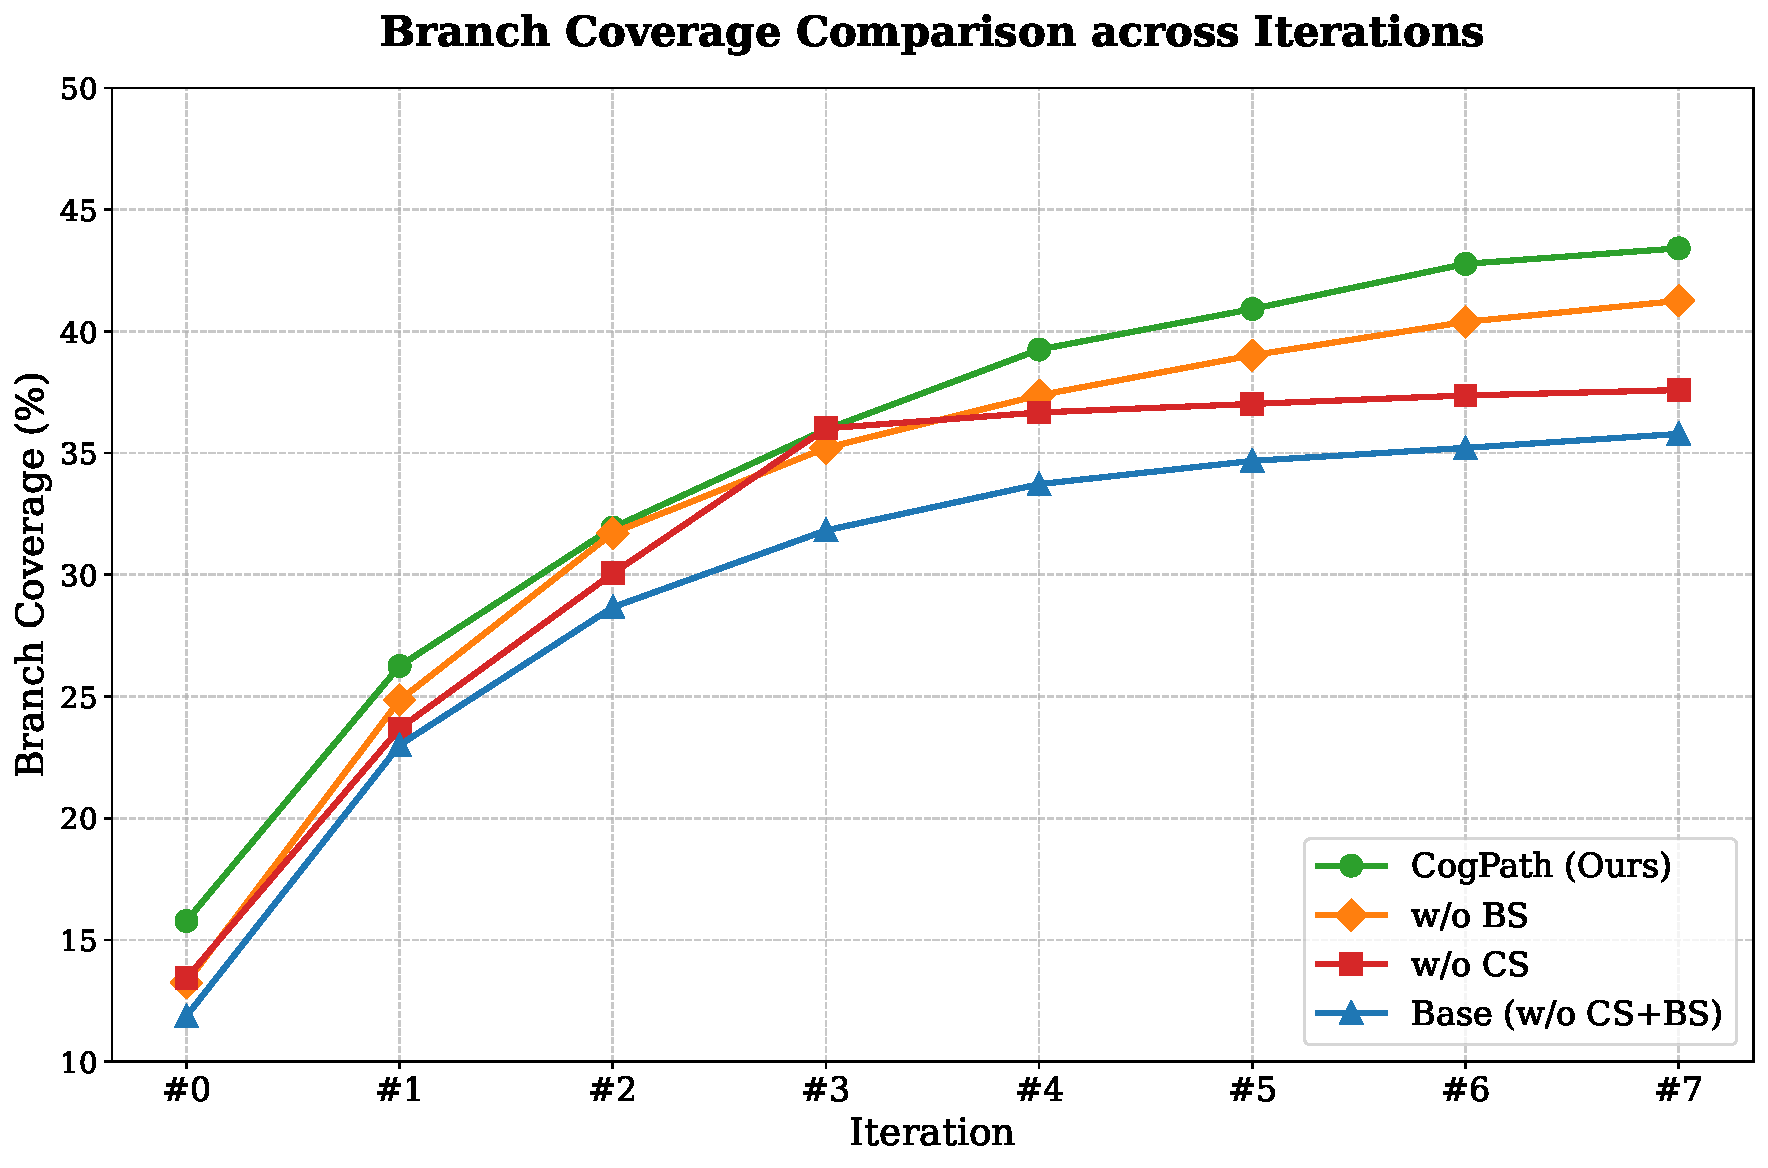
\includegraphics[width=\linewidth]{figures/branch_coverage_comparison.pdf}
    \caption{Branch coverage improvement over iterations for \ourmethod{} and its three ablated variants.}
    \label{fig:branch-growth}
\end{figure}

Figure~\ref{fig:branch-growth} traces branch coverage across iterations for all four configurations. \ourmethod{} consistently achieves the highest coverage at every iteration and exhibits the steepest growth curve, demonstrating that both BS and CS contribute not only to final coverage but also to the efficiency of iterative improvement. In contrast, removing either component leads to slower convergence, and removing both produces the flattest growth trajectory, underscoring the necessity of each component for sustained progress.

\begin{tcolorbox}[colback=gray!5, colframe=gray!100, title=Answer to RQ2]
Both BS and CS make independent and complementary contributions to \ourmethod{}. BS provides the larger share of improvement by eliminating irrelevant context ($-$5.94 pp when removed), while CS explicitly guides the LLM toward satisfying cross-method preconditions ($-$4.62 pp when removed). Removing both components degrades BC by 7.84 pp on average, with per-project drops reaching up to 27.49 pp (\textit{Csv}), confirming that neither component is redundant. The iterative growth curves further show that both components contribute to the efficiency of coverage accumulation across generation rounds.
\end{tcolorbox}

\subsection{RQ3: Performance Comparison of Different LLMs}
\begin{table*}[t]
\centering
\caption{Model Generalization Across Different LLMs}
\label{tab:model-generalization}
\small
\begin{tabular}{@{} l c c c c c c c c c c @{}}
\toprule
\multirow{2}{*}{Project} & \multirow{2}{*}{\#C} & \multirow{2}{*}{CC} &
\multicolumn{2}{c}{QC3-30B} & \multicolumn{2}{c}{GPT-5.4-Mini} & \multicolumn{2}{c}{QW3.5-397B} & \multicolumn{2}{c}{DS-V3.1} \\
\cmidrule(lr){4-5} \cmidrule(lr){6-7} \cmidrule(lr){8-9} \cmidrule(lr){10-11}
& & & LC(\%) & BC(\%) & LC(\%) & BC(\%) & LC(\%) & BC(\%) & LC(\%) & BC(\%) \\
\midrule
Cli & 2 & 11.00 & 84.32 & 70.73 & 97.86 & 86.18 & 98.82 & 92.63 & 98.82 & 91.93 \\
Codec & 7 & 16.14 & 76.97 & 69.60 & 89.78 & 82.61 & 98.32 & 95.30 & 93.60 & 88.46 \\
Collections & 5 & 18.60 & 40.46 & 34.63 & 98.31 & 94.14 & 98.16 & 94.43 & 98.02 & 94.20 \\
Compress & 9 & 15.33 & 36.09 & 29.05 & 87.15 & 80.29 & 86.92 & 80.90 & 81.32 & 76.04 \\
Csv & 3 & 16.67 & 62.27 & 52.29 & 87.42 & 77.76 & 95.71 & 87.42 & 85.70 & 77.53 \\
Gson & 4 & 23.25 & 63.82 & 41.24 & 90.26 & 83.06 & 92.88 & 87.97 & 92.13 & 82.86 \\
JCore & 9 & 16.33 & 41.72 & 35.54 & 63.71 & 57.83 & 83.25 & 76.77 & 66.62 & 57.76 \\
JDatabind & 9 & 15.33 & 23.35 & 17.85 & 76.16 & 68.78 & 74.93 & 69.81 & 84.06 & 77.44 \\
JXml & 4 & 21.50 & 20.61 & 17.08 & 73.41 & 74.20 & 62.20 & 63.65 & 66.06 & 65.22 \\
Jsoup & 8 & 14.13 & 66.43 & 52.55 & 93.37 & 82.96 & 95.87 & 87.49 & 87.15 & 79.98 \\
JxPath & 12 & 15.50 & 42.28 & 35.84 & 81.72 & 75.11 & 71.30 & 66.22 & 76.89 & 73.21 \\
Lang & 17 & 16.88 & 59.21 & 52.14 & 90.65 & 84.32 & 91.72 & 87.44 & 88.21 & 85.02 \\
Math & 30 & 16.47 & 59.60 & 54.02 & 88.89 & 81.82 & 92.96 & 87.47 & 91.69 & 85.41 \\
Time & 11 & 17.36 & 66.79 & 59.25 & 94.18 & 87.63 & 96.94 & 91.08 & 94.71 & 89.92 \\
\midrule
\multicolumn{3}{l}{Average} & 53.14 & 44.41 & 86.63 & 79.76 & 88.57 & 83.47 & 86.07 & 80.36 \\
\bottomrule
\end{tabular}
\end{table*}


Table~\ref{tab:model-generalization} reports LC and BC achieved by \ourmethod{} under four LLMs across all 14 projects. We discuss the results from three perspectives.

\noindent\textbf{Overall generalizability.}\ourmethod{} delivers consistently strong performance regardless of the underlying LLM, confirming that its coverage gains derive from the structural guidance of BS and CS rather than from any model-specific behavior.The three large-scale models—GPT-5.4-Mini, QW3.5-397B, and DS-V3.1—achieve average BC of 79.76\%, 83.47\%, and 80.36\%, respectively, whereas QC3-30B reaches 44.41\%.Despite this gap, QC3-30B already outperforms all baselines in RQ1 (best competitor: HITS at 34.24\%), demonstrating that \ourmethod{}'s framework-level contributions are effective even under limited model capacity.

\noindent\textbf{Interaction between model capacity and cyclomatic complexity.}The performance gap between QC3-30B and large models is not uniform across projects but is strongly modulated by cyclomatic complexity and inter-method dependency depth.On \texttt{Collections} (CC$_{avg}$ = 18.60), QC3-30B achieves only 34.63\% BC, while all three large models reach $\sim$94\%, a gap of nearly 60 pp.Similarly, on \texttt{Gson} (CC$_{avg}$ = 23.25, the highest in the benchmark), the gap exceeds 40 pp.In contrast, on lower-complexity projects such as \texttt{Cli} and \texttt{Time}, the gap narrows to under 20 pp, suggesting that \ourmethod{}'s structural guidance can partially compensate for limited model capacity when branch conditions are relatively straightforward.This pattern indicates that the primary bottleneck for QC3-30B is not the framework structure but the model's inability to perform the multi-step object initialization required by complex preconditions—precisely the reasoning that Constraint-Hints is designed to elicit.

\noindent\textbf{Synergy between Constraint-Hints and model reasoning capacity.}Cross-referencing with the ablation results in RQ2, CS contributes most on projects with deep cross-method dependencies (e.g., \texttt{JDatabind}: $-$8.52 pp when removed).These are also the projects where the capacity gap between QC3-30B and large models is most pronounced.This co-occurrence suggests a synergistic relationship: Constraint-Hints provides the LLM with explicit preconditions, but fully exploiting these hints requires multi-step reasoning capabilities that only sufficiently large models possess.In other words, CS lowers the reasoning barrier, while larger models are better positioned to clear it.

\noindent\textbf{Residual challenges across all models.}Despite the strong overall performance of large models, certain projects remain challenging regardless of model capacity.On \texttt{JCore} and \texttt{JXml}, the best-achieved BC across all large models stays below 77\% and 75\%, respectively.Manual inspection indicates that these projects contain deeply nested control flows where backward slicing occasionally produces overly coarse slices, inadvertently removing type information required for mock construction—a limitation identified in RQ2 that persists under stronger models.Furthermore, project-level variation among large models exists: on \texttt{JXml}, GPT-5.4-Mini (74.20\%) outperforms QW3.5-397B (63.65\%), while on \texttt{JCore}, DS-V3.1 (57.76\%) falls behind QW3.5-397B (76.77\%).Such sensitivity likely reflects model-specific differences in handling ambiguous or incomplete type hierarchies, which represents an avenue for future investigation.

\begin{tcolorbox}[colback=gray!5,colframe=gray!100, title=Answer to RQ3]
\ourmethod{} generalizes robustly across LLMs of varying scales and architectures.Model capacity plays a critical role: large-scale models outperform QC3-30B by up to 59.5 pp in BC, with the gap most pronounced on high-complexity projects requiring multi-step reasoning—precisely where Constraint-Hints provides the most structural guidance.Nonetheless, even QC3-30B surpasses all baselines in RQ1, confirming that \ourmethod{}'s framework-level design contributes independently of model capacity.Among large models, performance is broadly comparable, though residual challenges on projects with coarse-grained slicing sensitivity point to opportunities for further refinement.
\end{tcolorbox}

\section{DISCUSSION}

\ourmethod{} incurs additional prompting overhead due to backward slicing and constraint hint construction. On average, each focal method consumes approximately \textbf{43,000 tokens}, reflecting both the input code context and the appended constraints. Across all 3,576 requests in our evaluation, this corresponds to roughly \textbf{1.43 billion input tokens} and \textbf{12.5 million output tokens}, for a total of about \textbf{1.55 billion tokens}. The backward slicing step helps mitigate this cost by removing irrelevant statements, reducing the prompt length by roughly \textbf{25\%} before constraint hints are appended. In absolute terms, a project with 130 focal methods costs about \textbf{\$100}, which is reasonable considering the resulting coverage improvements.

\textbf{Token Efficiency.} Despite the large aggregate token consumption, \ourmethod{} achieves a favorable coverage-per-token ratio by focusing the LLM on relevant code slices and explicit constraints. This ensures that each token contributes meaningfully to exercising complex branches, improving the overall efficiency of test generation compared to naive full-context prompts.

\textbf{Qualitative Insight.} To illustrate why \ourmethod{} outperforms baseline approaches, we examine a representative example from the \textit{Favicon for Alibaba} project. The method \texttt{generateFavicon} contains a target branch condition \texttt{if (icon != null \&\& icon.size() > 0)}, which can only be satisfied if the object is properly initialized beforehand. Baselines generate tests that invoke the focal method directly, failing to establish the required state and leaving the branch uncovered. \ourmethod{}, by applying backward slicing, identifies the relevant state-setting call \texttt{setIconState} and provides a constraint hint specifying the precondition. The resulting test correctly initializes the object state and triggers the target branch. This example demonstrates that \ourmethod{}’s benefits extend beyond quantitative gains: it enhances the LLM's capacity to reason about cross-method dependencies in realistic Java programs.

\textbf{Limitations.} Despite its effectiveness, \ourmethod{} has notable constraints. \emph{Slice granularity.} For projects such as \textit{Collections} and \textit{Compress}, where branches depend on simple value-range conditions rather than cross-method state, the backward slice may remove auxiliary type or range information, reducing test quality. Conversely, overly coarse slices may retain irrelevant statements, introducing noise. Developing adaptive slicing strategies that adjust granularity based on branch type remains future work. \emph{Scalability.} Backward slicing and constraint extraction introduce preprocessing overhead proportional to the inter-procedural dependency graph. In our evaluation, average preprocessing time per focal method is \textbf{1.2\,s}, acceptable for medium-scale projects, though on-demand or incremental slicing may be required for industrial-scale codebases.

\section{RELATED WORK}

\subsection{Unit Test Generation}

Automated unit test generation has long been studied to reduce developer effort and improve software reliability. Existing techniques can be broadly categorized into search-based approaches and recent large language model (LLM)-based methods.

Search-based software testing (SBST) techniques construct test inputs by optimizing coverage objectives. A representative system is EvoSuite~\cite{evosuite}, which employs evolutionary algorithms to generate JUnit test suites that maximize structural coverage metrics such as branch coverage. EvoSuite adopts whole-test-suite optimization and regression assertion generation to capture program behavior automatically. Although SBST techniques are effective at exploring input spaces, they often struggle with complex semantic dependencies and may produce tests that are difficult for developers to interpret~\cite{mcminn2011}.

The emergence of large language models has enabled a new class of approaches that synthesize tests directly from source code. ChatUniTest~\cite{chen2024} leverages LLMs to generate unit tests using a focal-context mechanism that selectively exposes relevant program information to the model, combined with a generate–validate–repair workflow to improve compilation and execution success rates. SymPrompt~\cite{ryan2024} explores prompt engineering strategies that decompose test generation into structured reasoning steps aligned with program execution paths, enabling the model to better utilize type and dependency information.

Several recent studies further investigate how structured prompting can guide LLMs toward generating more effective tests. HITS~\cite{wang2024c} introduces a hierarchical prompting strategy that organizes test generation into multiple reasoning stages, allowing the model to progressively reason about program structure and test construction. This design improves the model's ability to generate syntactically valid and semantically meaningful tests.

Other approaches integrate execution feedback to improve test reliability. CoverUp~\cite{pizzorno2024} and Panta~\cite{gu2025a} adopt workflows that combine LLM-based generation with compilation and execution signals to refine generated tests and improve coverage. These studies show that incorporating program feedback can significantly enhance the executability and effectiveness of generated test suites.

Another line of work focuses on practical tooling for developers. JUnitGenie~\cite{liao2025} leverages LLMs to automatically synthesize JUnit tests from source code and project context, providing an assistant that integrates test generation into development workflows.

Despite these advances, existing approaches still exhibit important limitations. Search-based methods primarily focus on input exploration and often fail to capture semantic dependencies across methods~\cite{yang2024telpa}, while LLM-based approaches typically rely on static prompting strategies that lack explicit reasoning about program constraints. These limitations motivate approaches that more tightly integrate program analysis with LLM reasoning to guide test generation.

% SymPrompt利用提取每个可能执行分支的条件，只收集“近似”约束，引导LLM生成合适单元测试。但是只有分支条件，缺少输入条件和上下文的约束
% HITS将被测函数切片，简化被测函数的圈复杂度，降低LLM理解复杂代码的难度，以此提高分支覆盖率。但是函数切片缺少一个标准，有可能遗漏上下文生成错误代码
% CoverUp将利用动态覆盖率报告反馈指导LLM生成高覆盖率的单元测试
% Panta采用一种静态分析与动态报告结合的混合单测生成方法
% JUnitGenie通过类型信息、控制流结构和数据依赖构建上下文


\subsection{Program Slicing}

Program slicing is a classical program analysis technique used to extract the subset of program statements that are relevant to a particular computation or variable~\cite{weiser1984}\cite{tip1995}. Traditional slicing techniques rely on static or dynamic dependency analysis to identify statements that influence the value of a program element at a specific program point~\cite{tip1995}. JavaSlicer~\cite{JavaSlicer}, for example, performs dynamic slicing for Java programs by tracking runtime data and control dependencies, enabling developers to isolate statements that contribute to specific execution behaviors. Such slicing techniques have been widely used in debugging, program comprehension, and software testing.

Recent work has explored learning-based approaches to overcome the limitations of traditional slicing. NSSlicer~\cite{yadavally2024} introduces a neural slicing framework designed for incomplete or partial programs. By leveraging neural models to predict relevant dependencies, NSSlicer can generate meaningful slices even when static analysis is insufficient or when the code lacks full contextual information. This demonstrates the potential of integrating learning-based techniques with traditional program analysis.

In the context of LLM-based unit test generation, some studies adopt simplified forms of program decomposition. For instance, HITS~\cite{wang2024c} divides complex programs into smaller code segments to reduce the cognitive load for the LLM during test generation. However, this process does not follow the traditional notion of program slicing based on data and control dependencies; instead, it primarily serves as a heuristic strategy to simplify the input context provided to the model.

In contrast, \ourmethod{} leverages classical program analysis concepts more directly. Specifically, we perform backward slicing starting from uncovered branch conditions to identify the statements that influence the required program state. The resulting slice captures the dependencies necessary to satisfy the target branch. By providing this focused slice to the LLM, \ourmethod{} enables the model to reason about the required preconditions and generate tests that establish the necessary object state, thereby improving branch coverage.

\section{Conclusion and Future Work}
We presented \ourmethod{}, an LLM-driven framework for automated unit test generation that addresses two complementary dimensions of cognitive misalignment: Constraint-Hints makes implicit cross-method preconditions explicit, while coverage-driven Backward Slicing eliminates irrelevant context to concentrate the model's attention on branch-relevant dependencies. Evaluated on 130 classes and 2{,}971 complex methods from 14 real-world Java projects, \ourmethod{} achieves 44.41\% average branch coverage, outperforming state-of-the-art baselines by 10.2\,pp and generalizing consistently across LLMs of varying capacity.

Future work will pursue two directions. First, we plan to extend the framework with adaptive slice granularity selection and broader constraint guidance for complex object-oriented initialization patterns. Second, to assess how \ourmethod{}'s structural guidance compares with general-purpose agentic test generation, we will integrate its ConstraintSolver and BackwardSlicer into OpenHands and evaluate the resulting agent on the same benchmark under the same backbone model. To ensure a like-for-like comparison, the agent will operate under the identical information budget used in this paper---restricted to the declaring class source and import statements, with no access to external documentation, web search, or project-level dependencies---so that any difference in coverage and per-class cost is attributable to the agentic loop rather than to an enlarged information frontier.


\section{Data Availability Statement}
The replication package, including the source code of \textsc{CogPath} and evaluation scripts, is available for review at \url{https://anonymous.4open.science/r/CogPath-447B}. 
A permanent DOI-backed archive will be provided upon acceptance.

\section*{Acknowledgments}

This work is supported by the Frontier Technologies R\&D Program of Jiangsu (BF2024059), and the National Natural Science Foundation of China (No. 92582201, 62572229).
%
%
Yuan Yao is the corresponding author.

\bibliographystyle{IEEEtran}
\bibliography{references}

\end{document}
